\documentclass[ngerman, a4paper]{scrartcl}
\usepackage[T1]{fontenc}
\usepackage[utf8]{inputenc}
\usepackage{lmodern, graphicx, pgfplots, caption, amsmath, amsfonts, amssymb, babel}
\pgfplotsset{width=\linewidth/5}
\pgfplotsset{every tick label/.append style={font=\tiny}}
\captionsetup{justification=raggedright,singlelinecheck=false}
\newenvironment{mygraph}[1][]{%
	\begin{tikzpicture}
		\begin{axis}[
			mark=none,
			axis lines=left,
			xlabel=$x$,
			ylabel=$f(x)$,
			legend pos=outer north east,
			grid=major,
			scale only axis,
			legend style={nodes={scale=0.4, transform shape}},
			restrict y to domain=-10:10,
			#1
			]
		}{%
		\end{axis}
	\end{tikzpicture}
}

\begin{document}
	\title{Lösungen für Übungsaufgaben Mathematik~1 für die Übung am 7.6.24}
	\author{Emanuel Schäffer}
	\maketitle
	\section*{Aufgabe 1}
	\noindent
	a)
	\begin{mygraph}
		\addplot[samples=100, domain=-5:5, mark=none] {1/(1+exp(-x))};
	\end{mygraph}
	\noindent
	b)
	\begin{mygraph}
		\addplot[domain=-4:2, samples=100] {1/(x-1)};
		\addplot[domain=2:6, samples=100] {1/(x-1)};
		\addplot[mark=*, only marks, mark size=1.5pt, color=blue] coordinates {(1,0)};
	\end{mygraph}
	\noindent
	c)
	\begin{mygraph}
		\addplot[domain=0:5] {x+4};
		\addplot[domain=-5:0] {(x+4)^2};
	\end{mygraph}
	d)
	\begin{mygraph}
		\addplot[domain=0:5] {(x-2)^2};
		\addplot[domain=-5:0] {(x+2)^2};
	\end{mygraph}
	\noindent
	e)
	\begin{mygraph}
		\addplot[mark=none] {abs(x)};
	\end{mygraph}
	\noindent
	f)
	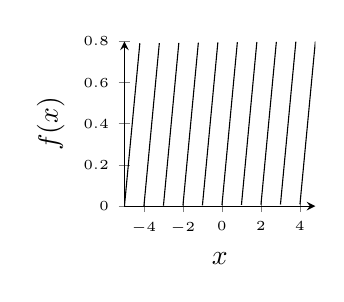
\begin{tikzpicture}
		\begin{axis}[
			axis lines=left,
			xlabel=$x$,
			ylabel=$f(x)$,
			legend pos=north west,
			%grid=major,
			scale only axis,
			legend style={nodes={scale=0.5, transform shape}},
			restrict y to domain=-0.8:0.8
			]
			\addplot[mark=none, samples=1000] {x-floor(x)};
		\end{axis}
	\end{tikzpicture}
	g)
	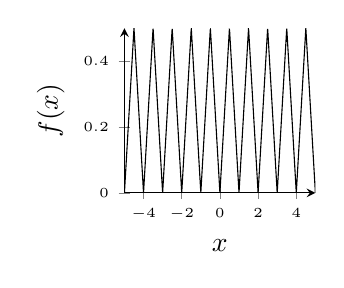
\begin{tikzpicture}
		\begin{axis}[
			axis lines=left,
			xlabel=$x$,
			ylabel=$f(x)$,
			legend pos=north west,
			%grid=major,
			scale only axis,
			legend style={nodes={scale=0.5, transform shape}},
			restrict y to domain=-10:10
			]
			\addplot[mark=none, samples=1000] {abs(floor(x+1/2)-x)};
		\end{axis}
	\end{tikzpicture}
	
	\section*{Aufgabe 4}
	\begin{tikzpicture}
		\begin{axis}[
			scale=2,
			axis lines=left,
			xlabel=$x$,
			ylabel=$f(x)$,
			legend pos=north west,
			scale only axis,
			axis lines=center,
			legend style={nodes={scale=0.5, transform shape}}
			]
			\addplot[mark=none, samples=1000, domain=-10:10] {x^5/100-30*x^3+1000*x};
		\end{axis}
	\end{tikzpicture}
	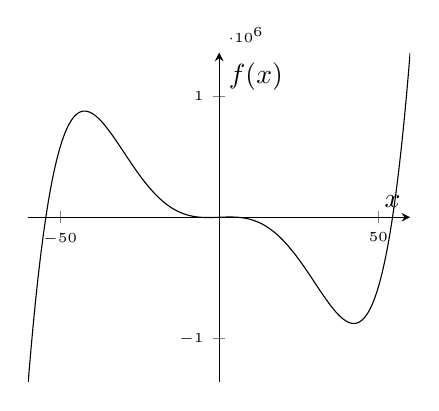
\begin{tikzpicture}
		\begin{axis}[
			scale=2,
			axis lines=left,
			xlabel=$x$,
			ylabel=$f(x)$,
			legend pos=north west,
			scale only axis,
			axis lines=center,
			legend style={nodes={scale=0.5, transform shape}}
			]
			\addplot[mark=none, samples=1000, domain=-60:60] {x^5/100-30*x^3+1000*x};
		\end{axis}
	\end{tikzpicture}
	
	\section*{Aufgabe 7}
	\begin{equation*}
		\begin{split}
			&\left({\begin{array}{ccc|c}
					10000&100&1&20\\
					40000&200&1&80\\
					48400&220&1&20
			\end{array}}\right)
			\vert 4\cdot I - II \quad \vert4.84\cdot I - III\\
			&\left({\begin{array}{ccc|c}
					10000&100&1&20\\
					0&-200&-3&0\\
					0&-264&-3.84&-76.8
			\end{array}}\right)
			\vert 1.32\cdot II - III\\
			&\left({\begin{array}{ccc|c}
					10000&100&1&20\\
					0&-200&-3&0\\
					0&0&0.12&-76.8
			\end{array}}\right)\\\\
			&0.12c = -76.8 \quad\vert :0.12\\
			&\underline{c = -640}\\
			&-200b-3\left(-640\right)=0 \quad\vert -1920 \quad\vert : -200\\
			&\underline{b=9.6}\\
			&10000a + 100\left(9.6\right) -640 = 20 \quad\vert -320 \quad\vert :10000\\
			&\underline{a=-0.03}\\
			&-0.03x^2+9.6x-640
		\end{split}
	\end{equation*}
	
	\section*{Aufgabe 8}
	\begin{equation*}
		\begin{array}{rrrrrl}
			x^4&-6x^3&-24x^2&-26x&-9&:(x+1)=x^3-7x^2-17x-9\\
			-(-x^4&+x^3)&&&&\\
			\cline{1-2}
			&-7x^3&-24x^2&&&\\
			&-(-7x^3&-7x^2)&&&\\	
			\cline{2-3}
			&&-17x^2&-26x&&\\
			&&-(-17x^2&-17x)&&\\
			\cline{3-4}
			&&&-9x&-9&\\
			&&&-(-9x&-9)&\\
			\cline{4-5}
			&&&&0&		
		\end{array}
	\end{equation*}
	\\
	
	\begin{equation*}
		\begin{array}{rrrrl}
			x^3&-7x^2&-17x&-9&:(x+1)=x^2-8x-9\\
			-(x^3&+x^2)&&&\\
			\cline{1-2}
			&-8x^2&-17x&&\\
			&-(-8x^2&-8x)&&\\	
			\cline{2-3}
			&&-9x&-9&\\
			&&-(-9x&-9)&\\
			\cline{3-4}
			&&&0&		
		\end{array}
	\end{equation*}
	
	$\Rightarrow x_{1-3}=-1, x_4=9$
	
\end{document}
